\section{Messmethoden}
\subsection{Anchor\/Beacon Nodes}

Als \textit{Anchor- oder Beacon Nodes} werden die Sensorknoten
bezeichnet, deren Position in einem globalen Koordinatensystem bekannt
sind. Diese Information kann auf zwei Weisen gewonnen werden. Zum ersten ist
es möglich, die Sensorknoten die als Ankerknoten fungieren sollen, 
mit einem GPS-Chip auszustatten und auf diese Weise die Position zu
jeder beliebigen Zeit zu ermitteln. Ein solcher Ansatz ist besonders
für den Fall sinnvoll, wenn der Ankerknoten oder sogar das gesammte
Sensornetz die Möglichkeit haben soll mobil zu sein. 

Die andere Möglichkeit besteht darin, die exakte Position des Ankerknotens fest einzuprogrammieren. Solch ein Ansatz ist empfehlenswert,
sollte das Sensornetz oder zumindest die Ankerknoten statisch sein. Der große Vorteil dieser Methode der vorprogrammierten Koordinaten ist,
das keinerlei zusätzlich Hardware am Sensorknoten angebracht werden muss und somit keine weiteren finanziellen Kosten anfallen und ebenso der
Energiebedarf der Knoten niedrig gehalten werden kann.
Um nun die Ankerknoten effektiv nutzen zu können benötigt man zur Erstellung eines globalen zweidimensionalen Koordinatensystems mindestens
drei Ankerknoten, welche nicht linear angeordnet sein dürfen. Soll sogar ein dreidimensonales globales Koordinatensystem erzeugt werden, wird
ein weitere Ankerknoten benötigt. Hier gilt die Einschränkung des zweidimensionalen Falles und zusätzlich muss der vierte Ankerknoten auf einer
anderen Ebene sein, als die anderen drei. Als sehr effektiv gilt hier
die Anordnung als Tetraeder.

Um nun unter Zuhilfenahme der Ankerknoten ein Koordinatensystem
aufbauen zu können, gibt es zwei Möglichkeiten. Zum einen ist es
realisierbar das  
ein mit Hilfe aller Sensorknoten erzeugtes relatives
Koordinatensystem, nachträglich auf Ankerknoten gelegt werden und
somit die relativen Positionen, in globale umrechenbar sind.
Andererseits ist es möglich die bekannten Positionen direkt bei den
Messungen zu nutzen und so, jede Position eines Sensorknotens direkt
als globale zu errechnen.

\subsection{Signalstärkemessung}
Die Signalstärkemessung oder \ac{RSSI} basiert auf der Idee, die bei einem kabellosen Sensornetz vorhandenen Sender und Empfänger zu nutzen um die 
Entfernung von Sensorknoten untereinander zu messen. Es wird davon ausgegangen das alle Sensorknoten eine identische Sendeleistung haben und es nun
möglich sein sollte über die ankommende Signalstärke exakt zu berechnen, wie weit der emittierende Sensorknoten vom empfangenden entfernt ist. Als 
physikalische Grundlage dient an dieser Stelle, das die Signalstärke im Vakuum, quadratisch zur zurückgelegten Entfernung abnimmt. In der Praxis 
hat sich allerdings herausgestellt das die Signalstärke durch aller Hand Störfaktoren, wie Luftfeuchtigkeit und -temperatur aber auch Störstrahlung 
und Hindernisse welche das Signal reflektiven oder absorbieren, beeinflusst wird. Die Abbildung \ref{fig:RSSI} zeigt das Ergebnis einer Messreihe und es 
wird hier deutlich, dass das reale Messergebnis in keiner Weise mit dem idealen kreisförmigen Ergebnis der Theorie übereinstimmt. \cite{whitehouse}

\begin{figure}[h!]
  \centering
  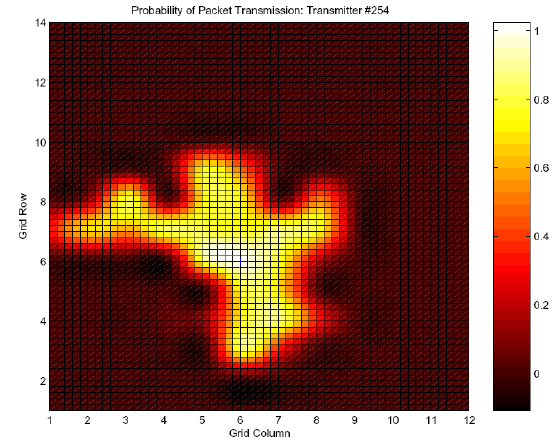
\includegraphics[scale=0.75]{img/RSSI1}\\
  \label{fig:RSSI}
  \caption{RSSI Meassurement}
\end{figure}

\subsection{Hop Count}
Die Messmethode des Hop Count basiert auf der Annahme, dass jeder Knoten der erreichbar ist, innerhalb der Sendereichweite R liegt. Die empfangene
Signalstärke spielt hierbei keine Rolle. Über alle Sensorknoten wird
ein ungerichteter Graph aufgebaut, wobei die Microcontroller die
Knoten sind und die Verbindungen der Sensorknoten die Kanten.

\begin{figure}[h!]
  \centering
  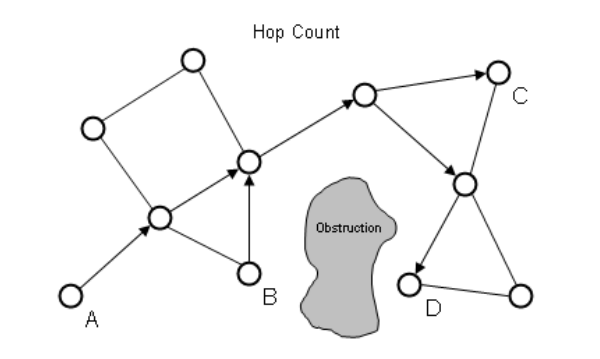
\includegraphics[scale=0.60]{img/hop_count1}
  \caption{Hop Count}
\end{figure}

\subsection{Zeitmessung}
Im Bereich der Zeitmessung werden hier drei Methoden vorgestellt. Im speziellen sind dies die \ac{ToA}, die \ac{TDoA} und die \ac{RToF}.
\subsubsection{Time of Arrival}
Die \ac{ToA} basiert auf der Berechnung des Zeitunterschieds zwischen Absenden und Empfang eines Signals. Als Berechnungsgrundlage wird hier
die Geschwindigkeit des Funksignals verwendet, die annähernd der Lichtgeschwindigkeit im Vakuum entspricht, hierraus kann dann einfach die 
Entfernung berechnet werden. Eine grafische Dartellung dazu wird in Abbildung \ref{fig:ToA} gezeigt. Diese Methode ist zwar äußerst genau, aber nur unter der Vorraussetzung, dass die Zeiten auf den beteiligten Sensorknoten absolut synchron laufen. Da dies nicht ohne weiteres zu bewerkstelligen ist, wurden verfeinerte Verfahren der Zeitmessung entwickelt, die ohne Synchronisation der einzelnen Knoten arbeiten können. 

\begin{figure}[h!]    
  \centering
  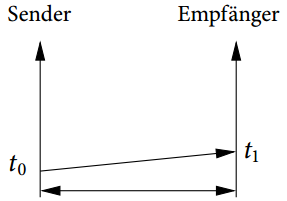
\includegraphics[scale=0.5]{img/time1}\\~\\
  \label{fig:ToA}
  $d = (t_{1} - t_{0}) \cdot c$\\
  $c=299\,792\,458\;\mathrm{m/s}$
  \caption{ToA}
\end{figure}

\subsubsection{Time Difference of Arrival}
Die \ac{TDoA} nutzt zur Umgehung des oben genannten Problems die
Tatsache, dass sich Schallwellen deutlich langssamer ausbreiten als
Funkwellen. Um dies zu nutzen werden alle Sensorknoten zusätzlich zur
Funkfähigkeit noch mit jeweils einem Mikrofon und einem Lautsprecher
ausgerüstet. Zur Messung wird nun zuerst per Funk ein Signal
abgesendet und nach einer fest definierten Pause, die auch 0 sein
kann, wird per Lautsprecher eine Tonfolge abgegeben. Nach dem beides
vom Zielknoten empfangen wurde, kann aus der Differenz der
Ankunftszeiten die Entfernung zum Senderknoten berechnet werden.
Hierfür nutzt man folgende Formel:

\begin{framed}
\begin{equation}
  \label{eq:TDoA}
    d = (s_{radio} - s_{sound}) * (t_{sound} - t_{radio} - t_{delay})
\end{equation}
\end{framed}
\myequations{Time Difference of Arrival: Entfernungsberechnung}

Die Hiermit ausgerechnet Entfernung ist sehr genau, unter der Vorraussetzung das zwischen Sender und Empfänger keinerlei Hinderniss existiert. Der große Nachteil dieser Messmethode ist der zusätzlich Bedarf an Hardware, welcher sowohl zu höheren Kosten als auch höherem Energieverbrauch führt. Ebenso werden die Sensorknoten durch die hinzugekommene Hardware größer.
\begin{figure}[h!]
  \centering
  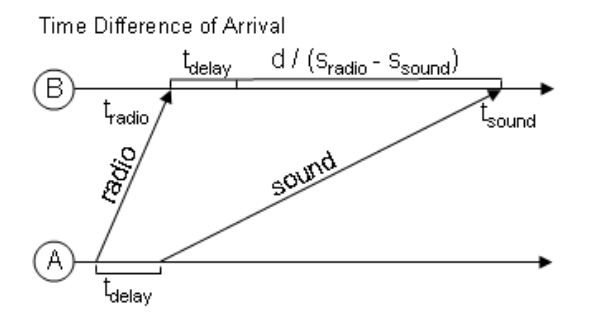
\includegraphics[scale=0.5]{img/tdoa1.png}\\
  \cite{bachrach}\\~\\
  $s_{radio}=299\,792\,458\;\mathrm{m/s}$\\
  $s_{sound}=          343\;\mathrm{m/s}$
  \label{fig:TDoA}
  \caption{TDoA}
\end{figure}

\subsubsection{Round Trip Time of Flight}
Die dritte und letzte Messmethode auf Basis der Zeitmessung die
vorgestellt wird, ist die \ac{RToF}. Bei dieser Methode wird bei der
ToA Methode nur der Funksender benötigt. Um das Problem der
Synchronisierung zu umgehen, wird das empfangene Funksignal zum Sender
nach einer vordefinierten Pause zurückgesendet. Über diese
Signallaufzeit kann nun die Entfernung wie folgt berechnet werden.

\begin{equation}
  \label{eq:RToF}
    d = \frac{t_{1} - t_{0} - t_{p}}{2} \cdot c
\end{equation}
\myequations{Round Trip Time of Arrival: Entfernungsberechnung}

Wobei $t_{1}$ der Empfangszeitpunkt am Sendeknoten, $t_{0}$ der
Sendezeitpunkt und $t_{p}$ die Länge der Pause zwischen Empfangs- und
Rücksendezeitpunkt des Signals am Empfängerknoten sind.
Grafisch ist dies in Abbildung \ref{fig:RToF} dargestellt.

\begin{figure}[h!]
  \centering
  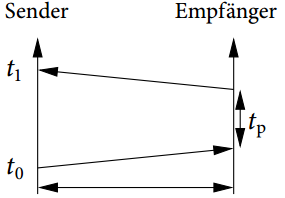
\includegraphics[scale=0.5]{img/time3}
  \label{fig:RToF}
  \caption{RToF}
\end{figure}
